\documentclass[main.tex]{subfiles}

\begin{document}
\sloppy


\vspace{1.0cm}

\section{Introduzione}\label{sec:Introduzione}
In tempi moderni, la rilevazione dei terremoti è diventata un tema fondamentale. Con l'aumento esponenziale della popolazione e la sua concentrazione nelle città, terremoti ad alta magnitudo potrebbero causare innumerevoli vittime. Purtroppo, i paesi in via di sviluppo, sono i più vulnerabili in  quanto spesso non dispongono di adeguate strutture antisismiche per prevenire il rischio di danni e perdite umane.
\begin{wrapfigure}{r}{0.25\textwidth}
    \centering
    \captionsetup{justification=centering}
    
\includegraphics[scale=0.15]{img/introduzione/seismocloud.png}
    \caption{Logo di SeismoCloud}
    \label{fig:seismologo}
\end{wrapfigure}
Come riportano molti ingegneri sismici: \say{earthquakes don’t kill people, collapsing buildings do}.\newline
Il progetto SeismoCloud ha l'obiettivo di usare una rete di sismometri per effettuare la rilevazione di terremoti, stimarne l'intensità e la provenienza e dare un allarme di preavviso ai dispositivi interessati.
\begin{quote}
Il progetto SeismoCloud\cite{SeismoCloud} nasce dalla collaborazione dell’Università 
 degli Studi di Roma \say{La Sapienza} e l’Istituto Nazionale di Geofisica e Vulcanologia. SeismoCloud è una rete comunitaria per la rilevazione dei terremoti e per l’invio di Early Warning, ovvero di avvisi che precedono (di alcuni secondi) l’arrivo di una scossa sismica. La rete funziona grazie a sismometri a basso costo sia fissi, costruiti come dispositivi dedicati, sia mobili, cioè basati su app per smartphone grazie all’uso dei sensori presenti nei dispositivi cellulari. 
Ogni persona può contribuire alla rilevazione dei terremoti installando l’app o montando e installando a casa un sismometro fisso. Tutti i sismometri sono registrati all’interno del cloud. Ogni volta che un sismometro rileva una vibrazione, che dipenda da un terremoto o no, la comunica via internet al server (cioè al computer centrale) di SeismoCloud. \newline
Il server, ricevendo le informazioni dei sismometri dal territorio ed eseguendo un algoritmo dedicato, è in grado di determinare il verificarsi di un terremoto nei primi secondi dall’inizio della scossa all’epicentro. Infatti, se si verifica un terremoto, i sismometri della zona dell’epicentro rilevano una vibrazione contemporaneamente. Se il numero di sismometri presente è sufficiente, il server registra il terremoto, ed effettua la stima dell’intensità della scossa e della distanza entro la quale il terremoto può provocare danni. In base a questa stima viene quindi inviato l’early warning, cioè la notifica sugli smartphone degli utenti delle province potenzialmente interessate.
\end{quote}

\subsection{I sismometri}
Un sismometro è un dispositivo di tracciamento e rilevamento delle vibrazioni. I moderni sismometri memorizzano i campioni in un formato digitale che può essere successivamente analizzato da un computer \cite{Seismometer}. E' possibile, inoltre, costruire il proprio sismografo, a basso costo, tramite le istruzioni presenti sul sito di SeismoCloud.\newline
Il progetto SeismoCloud è in grado di servirsi di smartphones come sismometri utilizzando gli accelerometri presenti per rilevare le vibrazioni, utilizzando l'apposita applicazione che è possibile scaricare dagli store.
\begin{figure}[H]
    \centering
    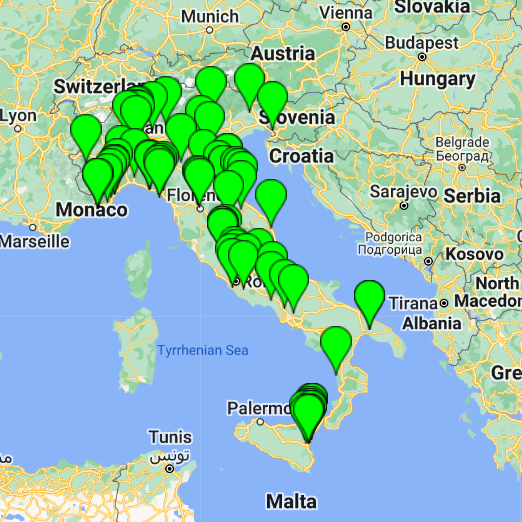
\includegraphics[width=1\linewidth]{img/introduzione/realtimemap2.png}
    \caption{Mappa in tempo reale dei sismografi nel suolo italiano}
    \label{fig:real-time-map}
\end{figure}

\subsection{Come si identifica un terremoto}
I sismometri che vengono utilizzati per eseguire la rilevazione dei terremoti risultano inaffidabili, se usati singolarmente, a causa delle vibrazioni prodotte dall'attività umana. Perciò, un grande numero di dispositivi consentirà di eseguire delle stime accurate; infatti, il verificarsi di un elevato volume di rilevamenti consentirebbe di stimare accuratamente l'arrivo di un terremoto.\newline
%I sismometri, data la loro inaccuratezza, non possono rilevare una scossa di terremoto. 
Il compito della rilevazione è delegata al server centrale, il quale raccoglie tutte le scosse provenienti dai sismometri e, grazie ad algoritmi dedicati al processamento delle \newline informazioni, riesce a calcolare se le scosse sono causate da un sisma.


\subsection{Percorso di tirocinio}
Come viene descritto nel sito del \say{Gamification Lab}, il percorso di tirocinio consiste in:
\begin{quote}
Ogni progetto è un gruppo di lavoro: quando si entra nel progetto da tirocinante/tesista si lavora in gruppo con altri studenti. In un primo periodo si inizierà a prendere confidenza con gli strumenti di lavoro e con il progetto, poi successivamente si passerà a piccoli lavori (risolvere piccoli bug, altri cambiamenti) ed infine, una volta preso “confidenza” con il progetto e con gli strumenti di lavoro, si sceglie un argomento specifico che costituisce il proprio lavoro di tirocinio/tesi.\cite{percorso-tirocinio}
\end{quote}


\subsection{Obiettivi del tirocinio}
Gli obiettivi principali del tirocinio sono stati il design e sviluppo di API, aggiunta di features e servizi.
\newline
Durante il periodo di tirocinio sono stati svolti i seguenti task:
\begin{itemize}
    \item Design e re-design di API
    \item Design e sviluppo di nuove funzionalità per migliorare l'esperienza all'interno\newline
    dell'applicazione
    \item Progettazione del sistema \say{\emph{post earthquake human presence detection}}
\end{itemize}

\subsection{Backend SeismoCloud}
Il backend del progetto SeismoCloud, consiste in diversi moduli che espongono vari servizi, ad esempio: webapi (espone le API per l'utente), worker (esegue diversi servizi periodici, come l'aggiornamento dei terremoti rilevati e l'aggiornamento di alcune statistiche), warehouse-worker (analizza i dati ricevuti dai sensori), warehouse-webapi (espone le API per raccogliere dati dai sensori).\newline
Il backend di SeismoCloud è scritto nel linguaggio di programmazione \say{Go} e fa uso di 2 database MariaDB e PostgreSQL. MariaDB viene utilizzato per la registrazione di informazioni riguardanti dispositivi e telefoni, messaggi di chat, impostazioni, dati relativi ai gruppi (vedi \ref{sec: gruppo}) e dati relativi, mentre PostgreSQL per archiviazione a lungo termine per dati come vibrazioni, intervalli di attività, temperatura, e dati affini. 
\subsection{Go}
Go\cite{go}, noto anche come Golang, è un linguaggio di programmazione \say{object oriented} open source compilato che supporta la tipizzazione statica. La sintassi di Go è stata progettata per essere semplice ed intuitiva; infatti Go utilizza il Garbage Collector (GC) per ottimizzare automaticamente l'utilizzo della memoria, evitando problemi comuni, come memory leaks, che hanno ad esempio altri linguaggi come \say{C} e \say{C++}. Go offre anche un meccanismo integrato per la concorrenza, basato sui canali (spiegati nel paragrafo \ref{sec:workerfdesign}), che consente di gestire in modo efficiente l'esecuzione di più attività contemporaneamente.\newline
In sintesi, Go è un linguaggio di programmazione moderno e innovativo che offre funzionalità avanzate come la gestione automatica della memoria e la concorrenza basata sui canali, rendendolo una scelta popolare per lo sviluppo di applicazioni ad alte prestazioni.

\subsection{Necessità del post earthquake human presence detection system}
Il sistema, allo stato attuale, effettua solo il rilevamento di terremoti anche grazie ad una rete di smartphones inviando, se necessario, un segnale di allerta.
\begin{quote}
    L’Early Warning del terremoto nelle zone limitrofe all’epicentro può essere ricevuto da 2 a 20 secondi prima dell’arrivo effettivo della scossa. L’early warning informa che c’è un terremoto in corso, e permette di mettersi subito al riparo, ad esempio sotto un tavolo, possibilmente anticipando l’arrivo della scossa sismica.\cite{SeismoCloud-EarlyWarning}
\end{quote}
Nonostante l'avviso permetta di ottenere del tempo prezioso per mettersi in sicurezza, non vi era modo di collezionare dati per aiutare le ricerche nel caso di disastri. Perciò si è pensato a un sistema e un protocollo da eseguire in seguito a terremoti ad alta magnitudo. Grazie a ciò è possibile ottenere informazioni sia senza sia tramite l'interazione con l'utente, potendo così offrire informazioni rilevanti e precise ai soccorsi.

\end{document}